%%%%%%%%%%%%%%%%%%%%%%%%%%%%%%%%%%%%%%%%%%%%%%%%%%%%%%%%%%%%%%%
%
% Welcome to writeLaTeX --- just edit your LaTeX on the left,
% and we'll compile it for you on the right. If you give
% someone the link to this page, they can edit at the same
% time. See the help menu above for more info. Enjoy!
%
%%%%%%%%%%%%%%%%%%%%%%%%%%%%%%%%%%%%%%%%%%%%%%%%%%%%%%%%%%%%%%%

% --------------------------------------------------------------
% This is all preamble stuff that you don't have to worry about.
% Head down to where it says "Start here"
% --------------------------------------------------------------
 
\documentclass[12pt]{article}
 
\usepackage[margin=1in]{geometry}
\usepackage{amsmath,amsthm,amssymb}

\usepackage{listings}
\usepackage{xcolor}
\usepackage{circuitikz}
\usetikzlibrary{bending}
\usetikzlibrary{patterns,decorations.pathmorphing,positioning}
\usepackage{float,graphicx}

%New colors defined below
\definecolor{codegreen}{rgb}{0,0.6,0}
\definecolor{codegray}{rgb}{0.5,0.5,0.5}
\definecolor{codepurple}{rgb}{0.58,0,0.82}
\definecolor{backcolour}{rgb}{0.95,0.95,0.92}

%Code listing style named "mystyle"
\lstdefinestyle{mystyle}{
  backgroundcolor=\color{backcolour}, commentstyle=\color{codegreen},
  keywordstyle=\color{magenta},
  numberstyle=\tiny\color{codegray},
  stringstyle=\color{codepurple},
  basicstyle=\ttfamily\footnotesize,
  breakatwhitespace=false,         
  breaklines=true,                 
  captionpos=b,                    
  keepspaces=true,                 
  numbers=left,                    
  numbersep=5pt,                  
  showspaces=false,                
  showstringspaces=false,
  showtabs=false,                  
  tabsize=2
}

%"mystyle" code listing set
\lstset{style=mystyle}

 
\newcommand{\N}{\mathbb{N}}
\newcommand{\Z}{\mathbb{Z}}
 
\newenvironment{theorem}[2][Theorem]{\begin{trivlist}
\item[\hskip \labelsep {\bfseries #1}\hskip \labelsep {\bfseries #2.}]}{\end{trivlist}}
\newenvironment{lemma}[2][Lemma]{\begin{trivlist}
\item[\hskip \labelsep {\bfseries #1}\hskip \labelsep {\bfseries #2.}]}{\end{trivlist}}
\newenvironment{exercise}[2][Exercise]{\begin{trivlist}
\item[\hskip \labelsep {\bfseries #1}\hskip \labelsep {\bfseries #2.}]}{\end{trivlist}}
\newenvironment{problem}[2][Problem]{\begin{trivlist}
\item[\hskip \labelsep {\bfseries #1}\hskip \labelsep {\bfseries #2.}]}{\end{trivlist}}
\newenvironment{question}[2][Question]{\begin{trivlist}
\item[\hskip \labelsep {\bfseries #1}\hskip \labelsep {\bfseries #2.}]}{\end{trivlist}}
\newenvironment{corollary}[2][Corollary]{\begin{trivlist}
\item[\hskip \labelsep {\bfseries #1}\hskip \labelsep {\bfseries #2.}]}{\end{trivlist}}

\newenvironment{solution}{\begin{proof}[Solution]}{\end{proof}}
 
\begin{document}
 
% --------------------------------------------------------------
%                         Start here
% --------------------------------------------------------------
 
\title{Lab 3}%replace X with the appropriate number
\author{Mengxiang Jiang\\ %replace with your name
CSEN 5303 Cybersecurity} %if necessary, replace with your course title
 
\maketitle
 
\begin{problem}{1} %You can use theorem, exercise, problem, or question here.  Modify x.yz to be whatever number you are proving
    Protecting Host Systems 

\begin{enumerate}
    \item On your virtual machine server, click the \textbf{Start} button, enter services, and launch the Services desktop app.
    \begin{figure}[H]
        \centering
        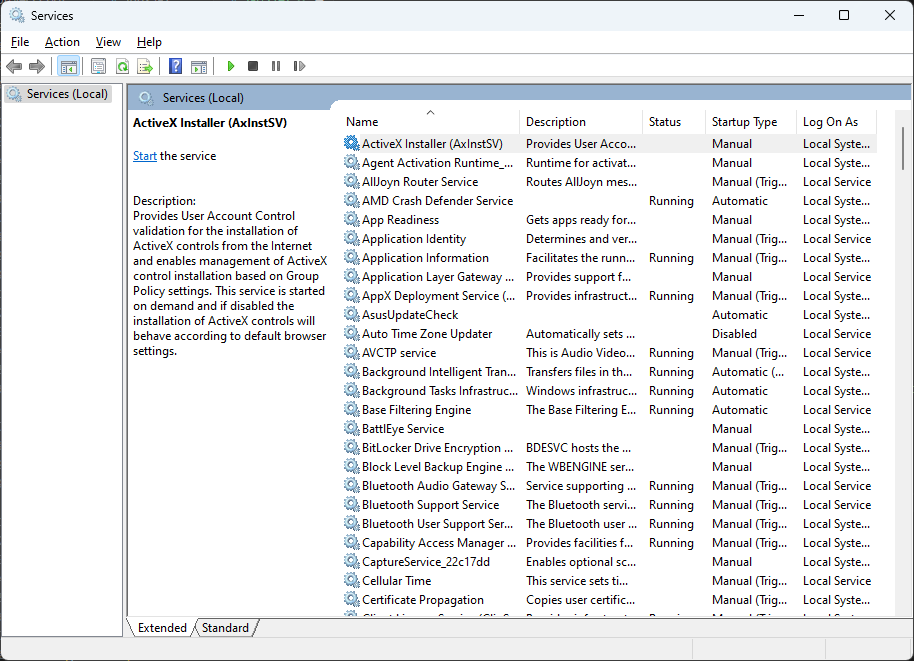
\includegraphics[width=0.7\textwidth]{services}
        \caption{Services screen}
    \end{figure}
    \pagebreak
    \item Practice sorting the columns by clicking each heading so you can view the services appropriately. Create
    and save two screenshots, each showing a differently sorted view.
    \begin{figure}[H]
        \centering
        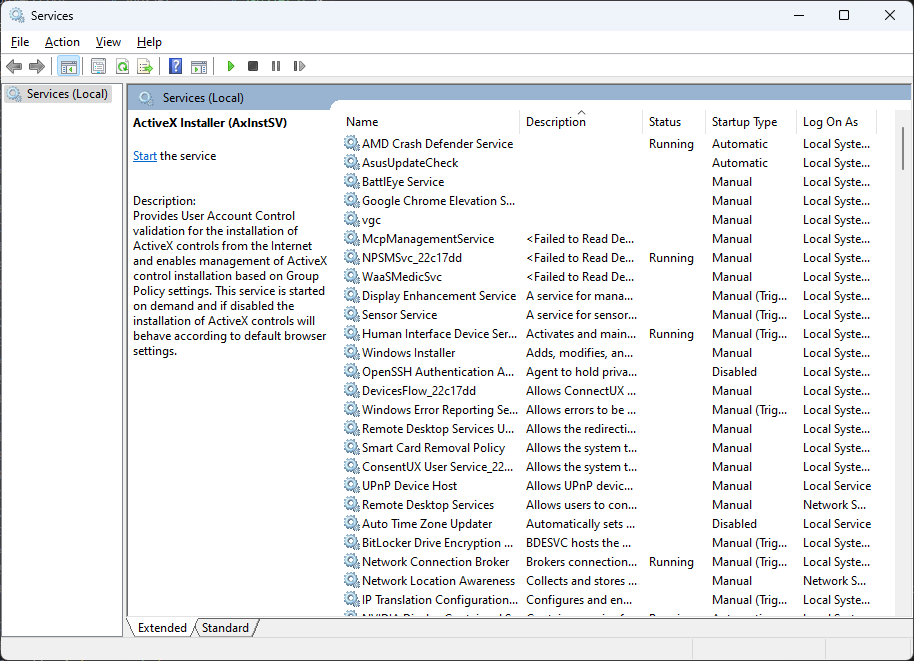
\includegraphics[width=0.7\textwidth]{services2}
        \caption{Services screen sorted by Description}
    \end{figure}
    \begin{figure}[H]
        \centering
        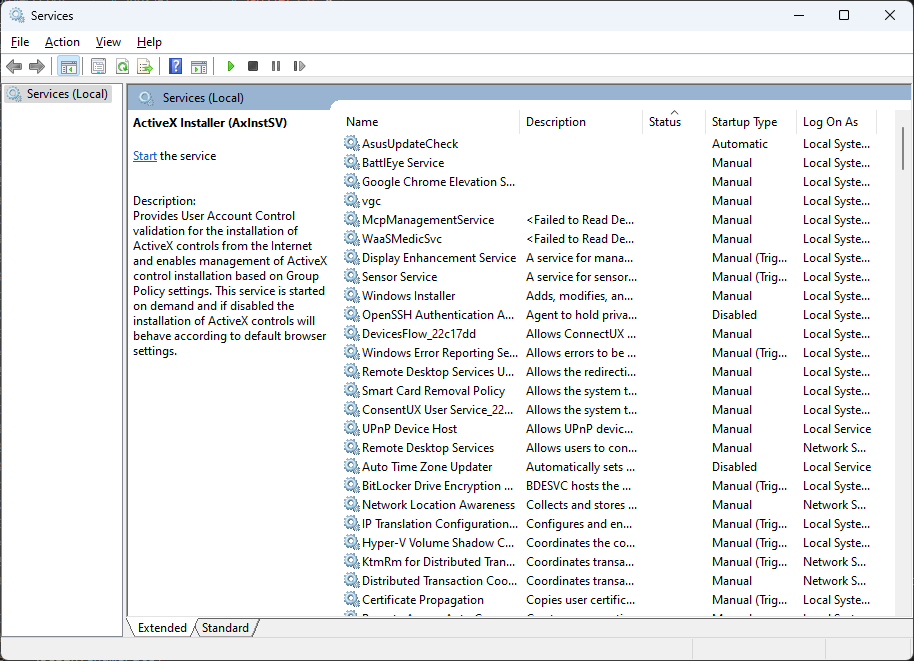
\includegraphics[width=0.7\textwidth]{services3}
        \caption{Services screen sorted by Status}
    \end{figure}
    \pagebreak
    \item Display the properties for the Task Scheduler service by double-clicking the service. What other programs
    would not run if this service is terminated?
    \begin{figure}[H]
        \centering
        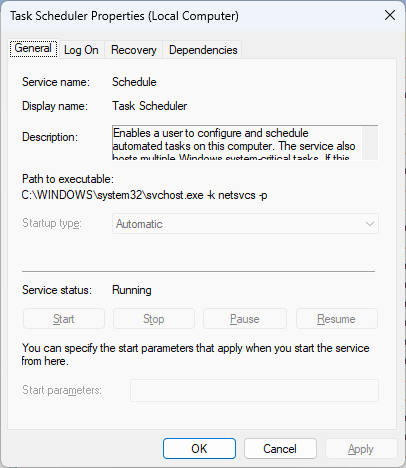
\includegraphics[width=0.45\textwidth]{task_scheduler_general}
        \caption{Task Schedular General properties}
    \end{figure}
    \begin{figure}[H]
        \centering
        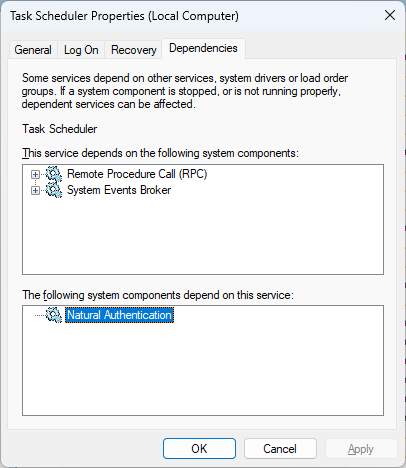
\includegraphics[width=0.45\textwidth]{task_scheduler_dependencies}
        \caption{Task Schedular Dependencies properties}
    \end{figure}
    Looks like the Natural Authentication service would not run if this service is terminated.
    \pagebreak
    \item What is the status of the Fax service?
    \begin{figure}[H]
        \centering
        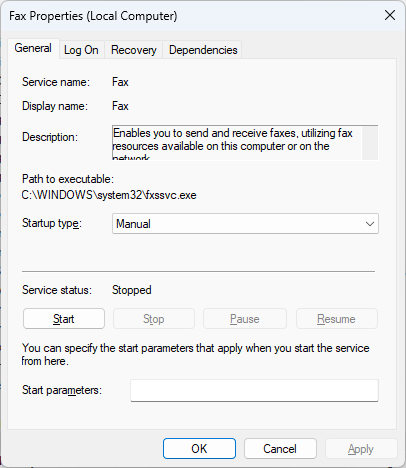
\includegraphics[width=0.45\textwidth]{fax_general}
        \caption{Fax General properties}
    \end{figure}
    The Fax service status is Stopped.
    \item In the properties for the Fax service, change the \textbf{Second failure}: setting to \textbf{Restart the Computer}. Create and save a screenshot of this setting. 
    \begin{figure}[H]
        \centering
        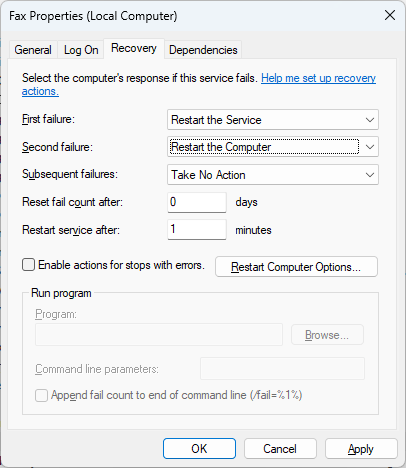
\includegraphics[width=0.45\textwidth]{fax_recovery}
        \caption{Fax Recovery properties}
    \end{figure}
\end{enumerate}

\end{problem}
% --------------------------------------------------------------
%     You don't have to mess with anything below this line.
% --------------------------------------------------------------
 
\end{document}